% !TeX root = ../dissertation.tex

\chapter{IMITATOR Backend for Uppex}
%\usepackage{tikz}

% Estilização do bloco EBNF
\tcbset{
  myebnf/.style={
    colback=blue!5!white, 
    colframe=blue!75!black, 
    fonttitle=\bfseries,
    title=Gramática do UppaalParser,
    sharp corners
  }
}

\tcbset{
  myebnf2/.style={
    colback=red!5!white, 
    colframe=red!75!black, 
    fonttitle=\bfseries,
    title=Gramática do ImitatorParser,
    sharp corners
  }
}
\usetikzlibrary{shapes.geometric, arrows, positioning}

% Estilo para os blocos e setas
\tikzstyle{class} = [rectangle, draw, rounded corners, minimum height=2em, align=left, font=\ttfamily, fill=blue!10]
\tikzstyle{abstractclass} = [class, fill=green!10, dashed]
\tikzstyle{trait} = [class, fill=red!10]
\tikzstyle{arrow} = [thick,->,>=stealth]

At this stage of the work, considering the capabilities demonstrated by the tools in the next chapter, the main focus is on integrating the tool with the UPPEX system. As mentioned in Chapter~\ref{ch:sota}, UPPEX allows extending an UPPAAL model through the use of annotated blocks and XML blocks. Previously, UPPEX only used UPPAAL as the model checker in the backend. However, with the integration of Imitator, it is now possible to have two backends: UPPAAL and Imitator. It is important to note that when using Imitator, only the presence of annotated blocks is required, which enhances the versatility and functionality of the tool. This integration opens up new possibilities for model checking, allowing users to choose between UPPAAL and Imitator based on their specific needs. Additionally, the flexibility to work with annotated blocks alone when using Imitator simplifies the modeling process while maintaining the robustness of the system. This means users can more easily extend their models and run checks with two powerful tools, optimizing performance and accuracy in different use cases. Additionally, this integration brought improvements to the Excel frontend, allowing it to handle the new Imitator syntax and support a new type of constraints and analyses, now enabling the use of parameters.

This chapter starts by presenting a simple example (the Coffee Machine) as a motivation for the new tool, before detailing the changes made to Uppex to accommodate the new backend and the resulting modifications. Finally, the previously referenced Worker-Hammer example will be used to demonstrate the functionality and results of the new version of Uppex.

%\begin{figure}[h]
%    \centering
%    \begin{standalone}
%        \begin{forest}
%            for tree={
%                font=\ttfamily,
%                grow'=0,
%                child anchor=west,
%                parent anchor=south,
%                anchor=west,
%                calign=first,
%                edge path={
%                    \noexpand\path [draw, \forestoption{edge}]
%                    (!u.south west) +(7.5pt,0) |- node[fill,inner sep=1.25pt] {} (.child anchor)\forestoption{edge label};
 %               },
 %               before typesetting nodes={
 %                   if n=1
%                      {insert before={[,phantom]}}
%                        {}
%                },
%                fit=band,
%                before computing xy={l=15pt},
%            }
%            [Main
%                [Backend
%                    [RunUppaal]
%                    [RunImitator, draw=red, thick]
%                ]
%                [Semantics
%                    [Annotations]
%                    [Configurations]
%                    [FeatureModel]
%                    [GenModel, draw=red, thick]
%                    [Uppaal]
%                    [Imitator, draw=red, thick]
%                ]
%                [Syntax
%                    [ExcelParser, draw=red, thick]
%                    [FeatExprParser]
%                    [Report]
%                    [UppaalParser]
%                    [ImitatorParser, draw=red, thick]
%                ]
%            ]
%        \end{forest}
%    \end{standalone}
%    \caption{Árvore de Estrutura}
%    \label{fig:tree}
%\end{figure}
% \section{Example: Coffee Machine}
\section{Quick Start Uppex with Imitator}

To download the new version of Uppex, the following steps must be followed:

\begin{itemize}
    \item \textbf{Access the official repository and select the latest version of the JAR file.}

    %colocar footnote
    Go to the official Uppex repository using the following \href{https://github.com/alexandre04032000/uppex-imitator/releases}{link} and select the recent version.

    \item \textbf{Ensure that Docker Desktop is running before executing the JAR file.}

    \item \textbf{Ensure that java is intalled}

    \item \textbf{Ensure that the excel file and xml/imi is in the same directory as the jar file}
\end{itemize}

%colocar footnote e refeir que se pode compilar o código fonte
These instructions are described in more detail in the official documentation of the tool, which has been upgraded to include the changes implemented in the new version and can be accessed through the following link: \url{https://github.com/alexandre04032000/uppex-imitator/blob/Uppex-Imitator/README.md}
\todo{use just the landing github page}
%codigo fonte mais instruções encontram-se na documentação e resumir os passos, dependencias e como correr/compilar
\section{Using Uppex with Imitator by example}
%esta secção running example to use throw this section

The model used to build the different configurations is the same as the one used in Chapter 3. It consists of three variables, all of which are parameters: $p_1$, the time between two consecutive sugar requests; $p_2$, the time interval during which the user can request sugar in the coffee; and finally $p_3$, the time required to complete the entire process of making and serving the coffee.

With this, we can construct four features: \textbf{Large, Small, Fast, Slow, Interval}. The first two refer to the time window during which the user can request sugar. Specifically, the Small feature represents a short interval both for making a sugar request and for the time between consecutive sugar requests. In contrast, the Large feature corresponds to longer intervals for both. The last two features are related to parameter $p_3$, representing the coffee preparation time: the Fast feature indicates a quicker preparation process, while the Slow feature indicates a longer one. It is important to note that all these features have predefined values. However, if different values are needed, they can be easily specified using the Interval feature.

Using these features, we built six configurations, as shown in Figure \ref{fig:cof_CM}: \textbf{Main, Large-Interval, Small-Interval, Fast-Coffee, Slow-Coffee, and Fixed-Coffee}. It is worth nothing that feature \textbf{Main} represents the original model without any modifications, with all three variables treated as parameters. In contrast, \textbf{Fixed-Coffee} represents a non-parametric model in which the interval for requesting sugar in the coffee is large, requiring the overall process to be fast—this is represented by the selection of the Slow-Coffee and Fixed-Coffee features.

\begin{figure}[H]
    \centering
    \begin{minipage}{0.5\textwidth}
        \centering
        \begin{tikzpicture}
            \node[anchor=south west,inner sep=0] (image1) at (0,0) {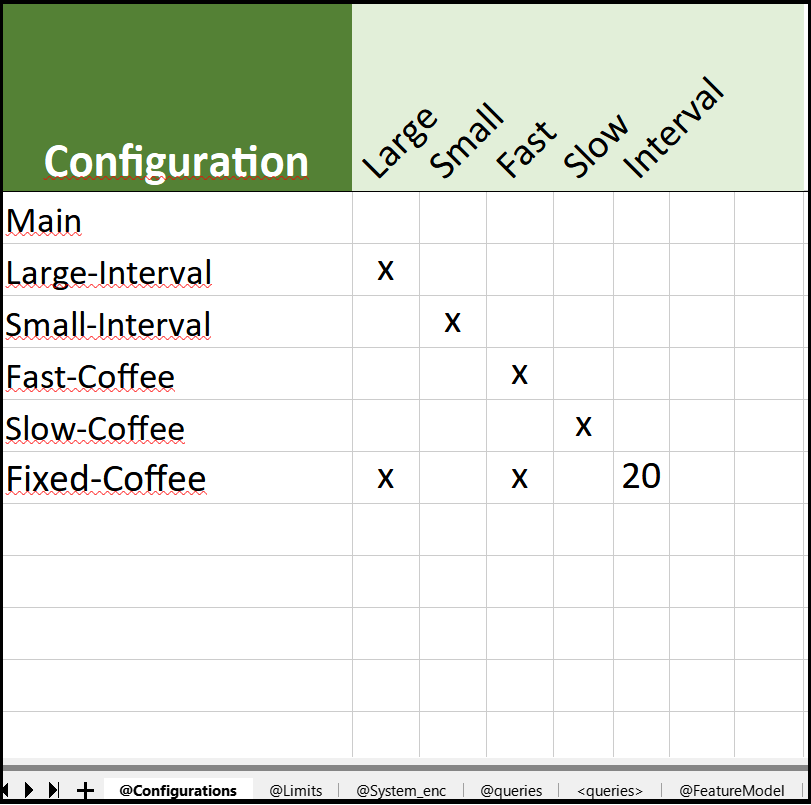
\includegraphics[width=0.8\linewidth]{images/new_example.png}};
            \begin{scope}[x={(image1.south east)},y={(image1.north west)}]
                \draw[black, thick] (0,0) rectangle (1,1); % coordenadas normalizadas
            \end{scope}
        \end{tikzpicture}
        \caption{Configurations Sheet Uppex}
        \label{fig:cof_CM}
    \end{minipage}
\end{figure}

It is necessary to construct the feature model in the corresponding sheet, as shown in Figure \ref{fig:cof_FM}, in order to constrain the feature selections and prevent combinations that do not make sense for the system in question.

\begin{figure}[H]
    \centering
    \begin{minipage}{0.5\textwidth}
        \centering
        \begin{tikzpicture}
            \node[anchor=south west,inner sep=0] (image1) at (0,0) {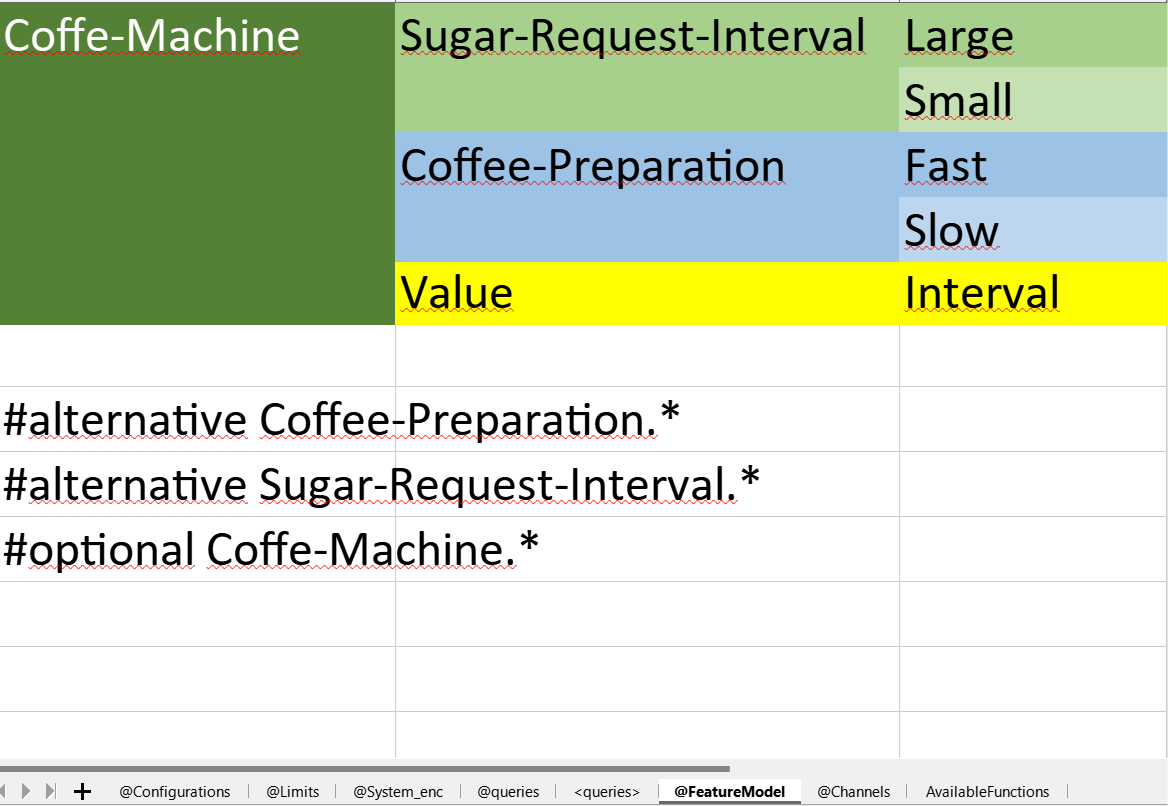
\includegraphics[width=0.8\linewidth]{images/new_FM.png}};
            \begin{scope}[x={(image1.south east)},y={(image1.north west)}]
                \draw[black, thick] (0,0) rectangle (1,1); % coordenadas normalizadas
            \end{scope}
        \end{tikzpicture}
        \caption{Feature Model Sheet Uppex}
        \label{fig:cof_FM}
    \end{minipage}
\end{figure}


We also built the Limits and System\_enc sheets, which represent the constraints applied to each parameter, as shown in Figures \ref{fig:PCSheetCM} and \ref{fig:LSheetsCM}, respectively.



\begin{figure}[H]
    \centering
    \begin{minipage}{0.48\textwidth}
        \centering
        \begin{tikzpicture}
            \node[anchor=south west,inner sep=0] (image1) at (0,0) {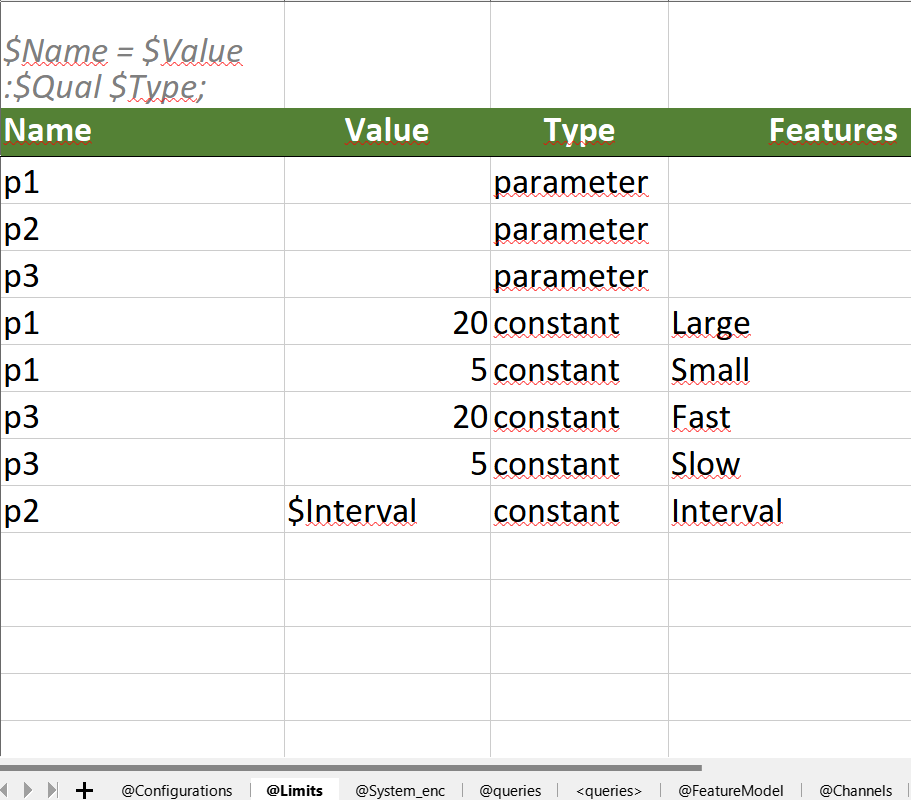
\includegraphics[width=\linewidth]{images/new_Lim.png}};
            \begin{scope}[x={(image1.south east)},y={(image1.north west)}]
                \draw[black, thick] (0,0) rectangle (1,1); % coordenadas normalizadas
            \end{scope}
        \end{tikzpicture}
        \caption{Limits Sheet}
        \label{fig:PCSheetCM}
    \end{minipage}
    \hfill
    \begin{minipage}{0.48\textwidth}
        \centering
        \begin{tikzpicture}
            \node[anchor=south west,inner sep=0] (image2) at (0,0) {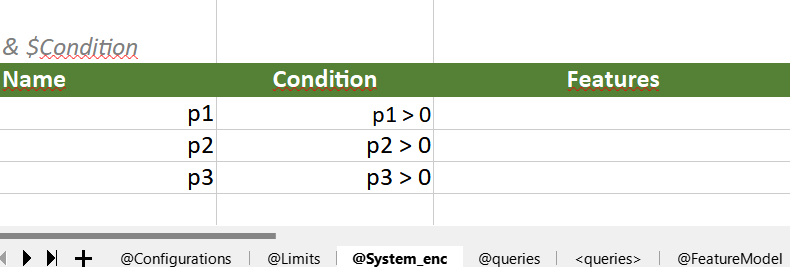
\includegraphics[width=\linewidth]{images/par_new.png}};
            \begin{scope}[x={(image2.south east)},y={(image2.north west)}]
                \draw[black, thick] (0,0) rectangle (1,1); % coordenadas normalizadas
            \end{scope}
        \end{tikzpicture}
        \caption{Parameters Constrain Sheet}
        \label{fig:LSheetsCM}
    \end{minipage}
\end{figure}

Finally, we configured the Queries sheet (Figure \ref{fig:Q_CM}). For the sake of simplicity, all configurations are set to verify the Deadlock property. Additionally, although not shown in the figure, the synthesis mode (as explained in the previous chapter) is set to synth.

\begin{figure}[H]
    \centering
    \begin{minipage}{\textwidth}
        \centering
        \begin{tikzpicture}
            \node[anchor=south west,inner sep=0] (image1) at (0,0) {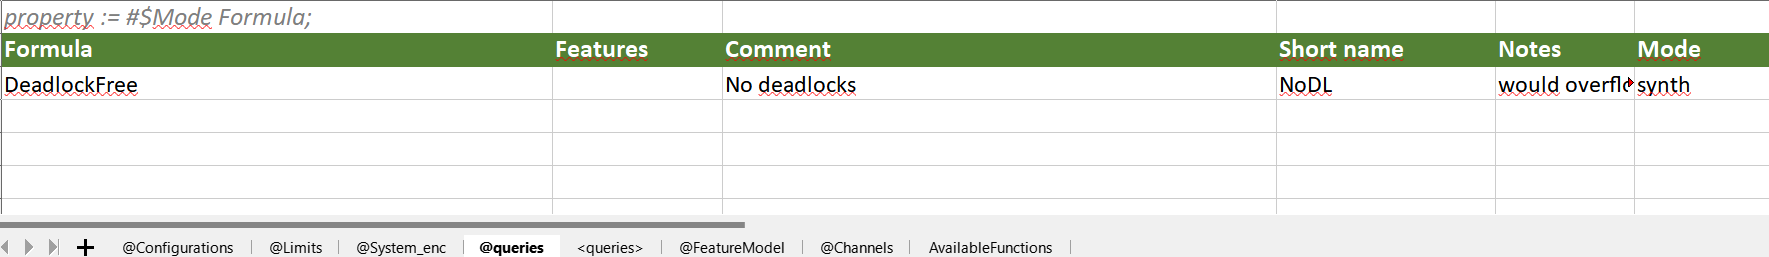
\includegraphics[width=\linewidth]{images/new_d.png}};
            \begin{scope}[x={(image1.south east)},y={(image1.north west)}]
                \draw[black, thick] (0,0) rectangle (1,1); % coordenadas normalizadas
            \end{scope}
        \end{tikzpicture}
        \caption{Queries Sheet Uppex}
        \label{fig:Q_CM}
    \end{minipage}
\end{figure}


With the parameterized model, we can run the JAR file, and the operating mode is exactly the same as the old version. Within the same directory, we need to have the JAR file and we can name it uppex.jar, the Excel file, and the Imitator file, with the last two files needing to have the same name.

In the terminal, we use the command: \texttt{java -jar uppex.jar -runAll Imitator\_Model.imi}, thus compiling all configurations. In each configuration, the deadlock property will be verified, and the results will be presented in an HTML file grouped by property and by configuration. For our example, the results can be found in Appendix C.\todo{use ref}

%discussion
As expected, for each of the configurations, in order for the property to be satisfied, $p_1$, $p_2$, and $p_3$ must fall within a specific range determined by the algorithm used. It is worth noting that the fixed\_coffee configuration does not have any associated interval since, as previously explained, all its variables are assigned fixed values. This turns it into a parametric model that, for the chosen values, verifies the condition. In this case, it reduces to the model checking of timed automata.

%motivating
% \section{Changes in UPPEX}
\section{Implementation details}
%colcoar intro
As previously mentioned, we will now provide a detailed explanation of the changes made to the old version of the tool to accommodate the new functionalities.
\subsection{Imitator Parser}
%alterar secções abaixo

To properly process and store the data extracted from Uppaal (.xml), Imitator (.imi), and Excel files, two specific data structures need to be created. These structures are designed to organize, structure, and simplify access to the collected information, ensuring efficient storage and data handling.

For reading Uppaal models, the solution to the problem is shown in the figure above in red. There is a base type called \textbf{Block} (like a code block), declared as a trait. Inside each block, there can be a tag (\textbf{NameBl}) that identifies the relevant part of the model, while the rest is called \textbf{content}.For this, two classes are created that extend this type, meaning they inherit its basic properties and behaviors, allowing them to reuse and specialize its functionalities. It is important to note that NameBl is written as an abstract class, meaning it cannot be instantiated directly and serves as a model for other classes that extend it. This means that NamedBl can define common methods and attributes but leaves the implementation of certain details to its subclasses. These are called \textbf{XmlElm}, if the tag is of the XML type, or \textbf{AnnotationBl}, when it is an annotation. Each of these subclasses specializes the behavior defined in the abstract class NamedBl, adapting to the specific type of block they represent. This ensures a clear distinction between XML elements and annotations, allowing proper handling for each case within the model. Along with the data structure, we also have a variety of helper functions aimed at displaying the model. 

In the constructors of the classes \texttt{NamedBl}, \texttt{XmElm}, and \texttt{AnnotationBl}, the following parameters are used:  

\begin{itemize}
    \item \textbf{\texttt{name}}: 
    
    Represents the name of the annotation.
    \item \textbf{\texttt{oldLines}}: 
    
    Contains the original content of the annotation, exactly as it appears in the source file.
    \item \textbf{\texttt{newLines}}: 
    
    Stores the updated content of the annotation, rewritten with the new values of the selected product. These values are formatted according to the structure specified in the first cell of the Excel file that matches both the name and type of the annotation.
\end{itemize}

To demonstrate how it works, we can consider the listing \ref{lst:imitator_example}, as an example. In this case, there is only one block with an annotation, specifically an annotation block of type \textbf{(Name)}, where the name is "Limits", corresponding to the \textbf{name} parameter in the constructor. The content of this block will be stored exactly as it is in the \texttt{oldLines} parameter.

To populate \texttt{newLines}, we need to refer to the Uppex Excel file. The Excel file contains a sheet with the same name as the annotation block, as shown in Figure \ref{fig:sheet}. Additionally, in the first cell of the sheet, we can find the structure that specifies how to construct each annotation block.

For instance, if we consider the product in question to be "lazy," then the annotation block is rewritten according to the structure defined in the Excel file. This rewritten block is displayed in listing \ref{lst:uppaal_example}. The Excel part will be detailed in the next chapter.



\lstdefinelanguage{UPPAAL}
{
    keywords={var, clock, discrete, bool, constant, parameter, automaton, sync, loc, invariant, when, do, goto, end, init},
    keywordstyle=\color{keywordcolor}\bfseries,
    % morecomment=[l]{(*},
    % morecomment=[r]{*)},
    commentstyle=\color{commentcolor}\textit,
    morestring=[b]",
    stringstyle=\color{stringcolor},
    basicstyle=\ttfamily\small,
    backgroundcolor=\color{backgroundcolor},
    tabsize=4,
    showstringspaces=false,
    breaklines=true
}


\definecolor{keywordcolor}{RGB}{0,0,255}      % Azul para palavras-chave
\definecolor{commentcolor}{RGB}{0,128,0}      % Verde para comentários
\definecolor{stringcolor}{RGB}{163,21,21}     % Vermelho escuro para strings
\definecolor{backgroundcolor}{RGB}{240,240,240}

\begin{figure}[H]
    \centering
    \begin{lstlisting}[language=UPPAAL, caption={Example of Imitator syntax}, label={lst:imitator_example},mathescape=true]
var
    session, t : clock;
    nails : discrete;
    b = True : bool;


(* @Limits *)
    sessionTime = 100 : constant;
    countNails = True : bool;
    infiniteNails = False : bool;   $\tikz[overlay, remember picture]{\coordinate(nails);}$
    reactTime = 20 : constant;
    totalNails : parameter;
    \end{lstlisting}
\end{figure}

% Creating arrows and explanations
\begin{tikzpicture}[overlay, remember picture]

Explanation box 1
\node[text width=5cm, draw, fill=white] (box1) at (12, 5.4) {
    \textbf{Annotation Block} \\
   \small Stored as Annotation Block named Limits
};
%%% Variation using the "nails" coordinate
% \node[text width=5cm, draw, fill=white,xshift=60mm] (box1) at (nails) {
%     \textbf{Annotation Block} \\
%    \small Stored as Annotation Block named Limits
% };

% Explanation box 2
\node[text width=5cm, draw, fill=white] (box2) at (12, 8.5) {
    \textbf{Content Block} \\
    \small Stored as Content Block
};

\draw[->, red, thick] (3.5,5.4) -- (box1.west);
% \draw[->, red, thick] (nails) -- (box1);
\draw[->, red, thick] (4.5,8.5) -- (box2.west);

\end{tikzpicture}

\begin{figure} [H]
    \centering
    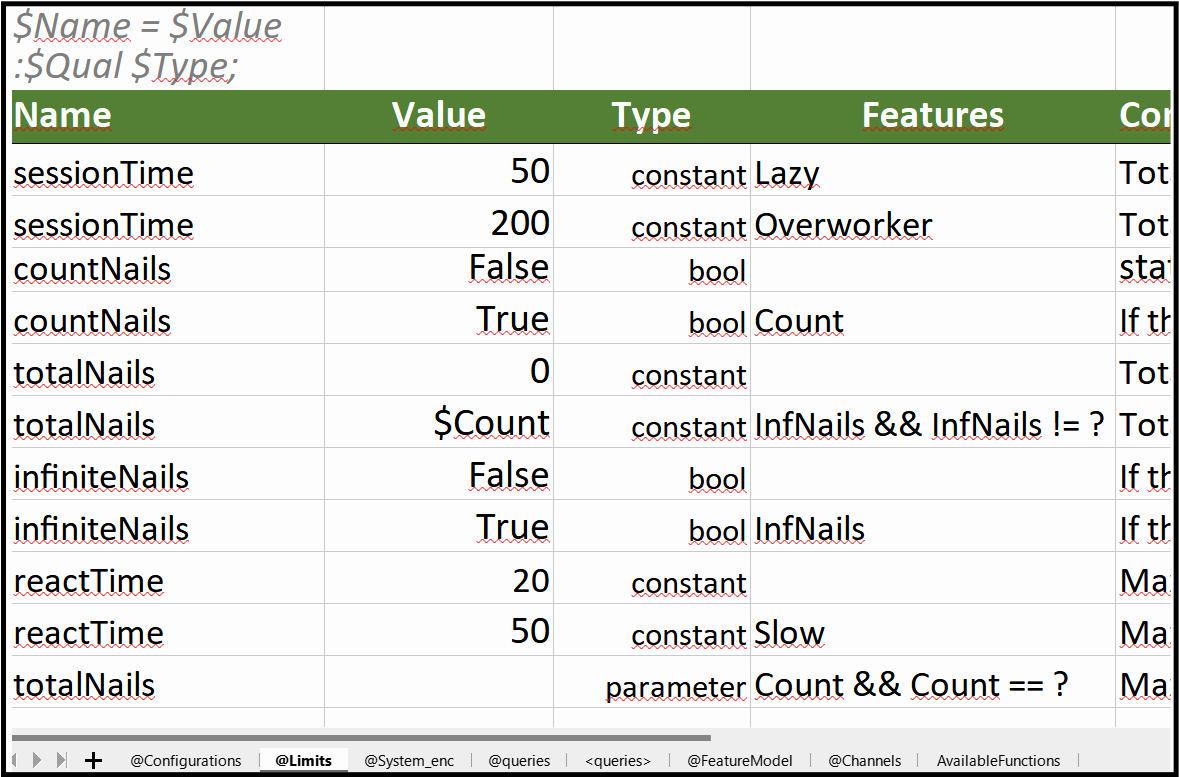
\includegraphics[width=0.75\linewidth]{images/uppex_imi.png}
    \caption{Limits Sheet from Uppex }
    \label{fig:sheet}
\end{figure}

\begin{figure}[H]
    \centering
    \begin{lstlisting}[language=UPPAAL, caption={Annotation Block rewritten with new values}, label={lst:uppaal_example}]
(* @Limits *)
    countNails = False : bool;
    sessionTime = 50 : constant;
    totalNails = 0 : constant;
    infiniteNails = False : bool;
    reactTime = 20 : constant;
    \end{lstlisting}
\end{figure}

%\vspace{1cm}


To better understand the Data structure, we built a class diagram, as shown in Figure \ref{fig:UPDS}.

\begin{figure}[H]
    \centering
    % \begin{standalone}
        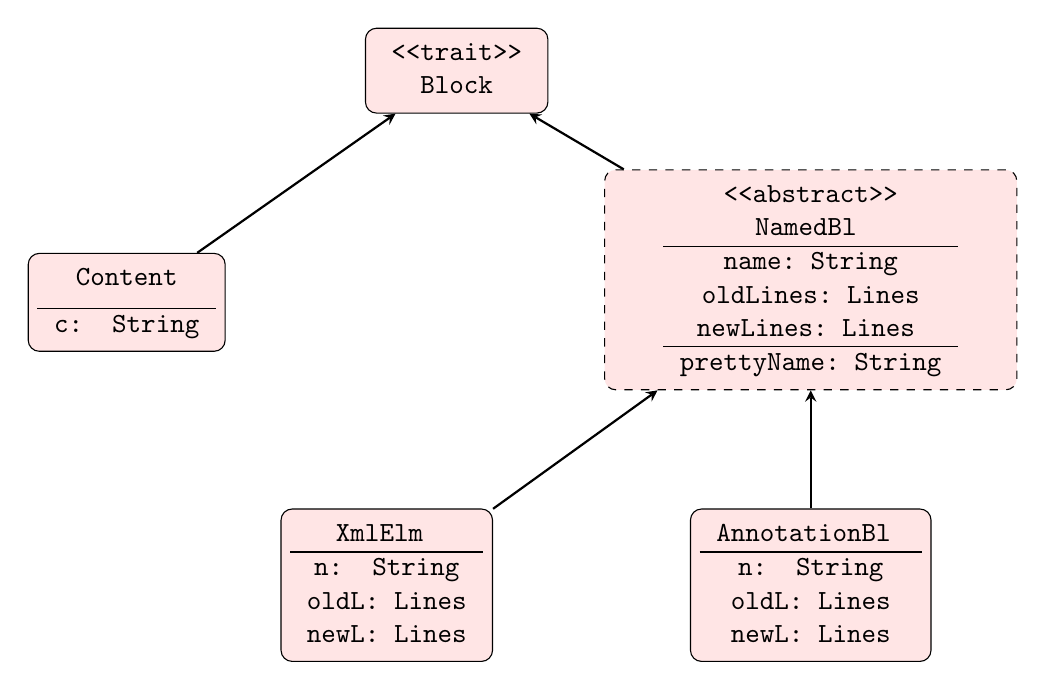
\begin{tikzpicture}[node distance=2.5cm, auto]
          % Nó para Block (sealed trait)
          \node (block) [trait,fill=red!10]
          {\begin{tabular}{c}
          <<trait>>\\
           \textbf{Block}
           \end{tabular}};
        % 
        % 
          % Nó para Content (classe concreta)
          \node (content) [class,fill=red!10, below left=of block]
          { \begin{tabular}{c}
            \textbf{Content} \\[1ex]\hline
            c: String
          \end{tabular}};
        % 
          % Nó para NamedBl (sealed abstract class)
          \node (namedbl) [abstractclass,fill=red!10, below right=1cm of block,text width=5cm, align=center]
          {\begin{tabular}{c}
            <<abstract>>\\
           \textbf{NamedBl}  ~\\\hline
           name: String \\ 
           oldLines: Lines \\ 
           newLines: Lines ~\\ \hline
           prettyName: String
           \end{tabular}};
        % 
          % Nó para AnnotationBl (classe concreta)
          \node (annotationbl) [class,fill=red!10, below=1.5cm of namedbl]
          {\begin{tabular}{c}\textbf{AnnotationBl} ~\\ \hline
           n: String \\ 
           oldL: Lines \\ 
           newL: Lines
           \end{tabular}};
        % 
          % Nó para XmlElm (classe concreta)
          \node (xmlelm) [class,fill=red!10, left=of annotationbl]
          {\begin{tabular}{c}\textbf{XmlElm} ~\\ \hline 
           n: String \\ 
           oldL: Lines \\ 
           newL: Lines
           \end{tabular}};
        % 
        % 
          % Conexões (relações de herança/implementação)
          %\draw [arrow] (Model) -- (GenModel);
          \draw [arrow] (content) -- (block);
          \draw [arrow] (namedbl) -- (block);
          \draw [arrow] (annotationbl) -- (namedbl);
          \draw [arrow] (xmlelm) -- (namedbl);
        \end{tikzpicture}
    % \end{standalone}
    \caption{Uppaal Parser Data Structure}
    \label{fig:UPDS}
\end{figure}

The data structure for Imitator will be very similar, allowing us to reuse the Uppaal structure. However, we can omit the XmlElm blocks, as they are no longer applicable, as shown in Figure \ref{fig:IPDS}.

\begin{figure}[H]
    \centering
    % \begin{standalone}
        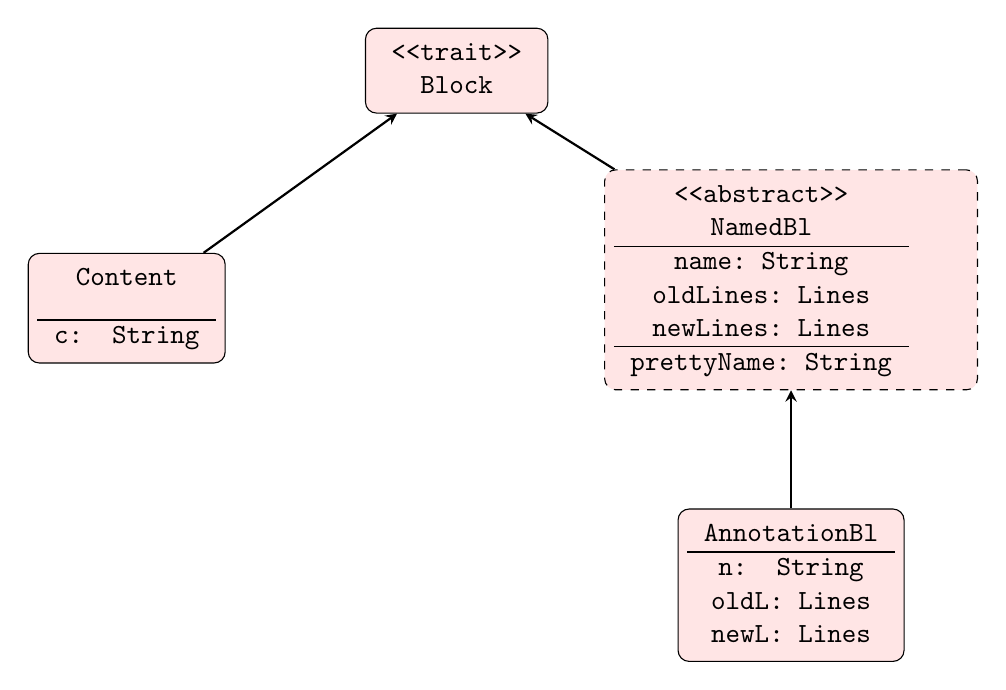
\begin{tikzpicture}[node distance=2.5cm, auto]
          % Nó para Block (sealed trait)
          \node (block) [trait,fill=red!10]
          {\begin{tabular}{c}
          <<trait>>\\
           \textbf{Block}
           \end{tabular}};
        % 
        % 
          % Nó para Content (classe concreta)
          \node (content) [class,fill=red!10, below left=of block]
          {\begin{tabular}{c}\textbf{Content} \\[3mm] \hline
           c: String
           \end{tabular}};
        % 
          % Nó para NamedBl (sealed abstract class)
          \node (namedbl) [abstractclass,fill=red!10, below right=1cm of block,text width=4.5cm]
          {\begin{tabular}{c}<<abstract>>\\
           \textbf{NamedBl} \\ \hline
           name: String \\ 
           oldLines: Lines \\ 
           newLines: Lines \\ \hline
           prettyName: String
           \end{tabular}};
        
          % Nó para AnnotationBl (classe concreta)
          \node (annotationbl) [class,fill=red!10, below=1.5cm of namedbl]
          {\begin{tabular}{c}\textbf{AnnotationBl}\\ \hline
           n: String \\ 
           oldL: Lines \\ 
           newL: Lines
           \end{tabular}};
% 
                % 
          % Conexões (relações de herança/implementação)
          %\draw [arrow] (Model) -- (GenModel);
          \draw [arrow] (content) -- (block);
          \draw [arrow] (namedbl) -- (block);
          \draw [arrow] (annotationbl) -- (namedbl);
        \end{tikzpicture}
    % \end{standalone}
    \caption{Imitator Parser Data Structure}
    \label{fig:IPDS}
\end{figure}


To expand the tool to support Imitator models while reusing code without adding unnecessary complexity(such as code duplication and the need to assign different names to identical code blocks), a trait with several abstract methods has been created. The functions responsible for rewriting code blocks that were previously defined only for UPPAAL will be implemented in the Imitator or Uppaal classes, which extend the trait. This will allow code reuse while maintaining the flexibility and modularity of the system.
This structure will also be reused, although, in the case of Imitator, the XmlElm block will not be used, as the tags inside < > will not be employed. This structure will now be part of a new singleton called GenModel and it is imported during the parsing of either the Uppaal or Imitator file, with the trait class also being declared in the same file and having the same name.



With the data structure set up, we need to build a parser to read the Imitator file, classifying each part according to the tags encountered. In parsing, code is taken from the preprocessor, broken into smaller pieces and analyzed so other software can understand it. The parser does this by building a data structure out of the pieces of input \cite{techtarget_parser}. 

Note that in the new version of Uppex, the notation that identifies the beginning of an annotation block for Imitator is in the form "$\textbf{(*Name of the Annotation Block*)}$".%, while the XML block remains the same as "\textbf{<Name of the XML Annotation Block>}". However, in the case of Imitator, the latter will not be used.


\newcolumntype{L}{>{\ttfamily}l}

\begin{table}[h]
    \centering
    \begin{tcolorbox}[colback=gray!10, colframe=black]
    \caption{Syntactic rules of the grammar}
    \label{tab:syntactic-rules_fin}
    \begin{tabular}{L L L}
        \textbf{Rule} & \textbf{::=} & \textbf{Definition} \\
        \hline
        annotationBlock & ::= & "(*" "@" anName "*)" [ newLine body ] \\
        lineBlock & ::= & line \\
        body & ::= & repsep(neLine, newLine) \\
    \end{tabular}
    \end{tcolorbox}
\end{table}

\begin{table}[H]
    \centering
    \begin{tcolorbox}[colback=gray!10, colframe=black]
    \caption{Basic tokens of the grammar}
    \label{tab:basic-tokens_fin}
    \begin{tabular}{L L L}
        \textbf{Token} & \textbf{::=} & \textbf{Definition} \\
        \hline
        newLine & ::= & \verb|\n| \\
        line & ::= & rep(word) \\
        neLine & ::= & rep1(word) \\
        word & ::= & \verb|[^\n]+| \\
        anName & ::= & \verb|[^*]+| \\
    \end{tabular}
    \end{tcolorbox}
\end{table}

The functioning of this parser is quite simple. We start by reading the file as a string and passing the result to the parse function, which in turn calls imitator, the main parser that splits the code into blocks. The syntactic rules used for this parsing process are shown in Table \ref{tab:syntactic-rules_fin}, while the basic tokens of the grammar are presented in Table \ref{tab:basic-tokens_fin}. The parser uses repsep(imitatorElem, newLine) to divide the content into lines or blocks. imitatorElem works as a block recognizer: if it finds (*@name*), it identifies it as an annotation(Annotation Block) and stores its name and content; otherwise, it considers the line as normal content (Content).

%\definecolor{keywordcolor}{rgb}{0.5,0.0,0.5}
%\definecolor{commentcolor}{rgb}{0.25,0.5,0.35}
%\definecolor{stringcolor}{rgb}{0.58,0.0,0.0}
%\definecolor{backgroundcolor}{rgb}{0.95,0.95,0.95}



%\begin{figure}[H]
%    \centering
%    \begin{standalone}
%        \begin{tikzpicture}[node distance=0.5cm, auto]
%            % Nó para GenModel (trait)
%          \node (GenModel) [trait,fill=green!10,text width=5cm] {
%          \centering <<trait>>\\
%          \centering \textit{\textbf{GenModel}} 
%%          \\[1ex] \\ \hline \\[1ex]
%          blocks: List[Block] \\[1ex] \\ \hline \\[1ex]
%          toString: String \\[1ex]
%          \textit{buildold} : \textit{String}  \\[1ex]
%          \textit{buildnew} : \textit{String}  \\[1ex]
%          \textit{build} : \textit{String}
%        };
        
        

%           \node (Imitator) [class,fill=green!10,text width=5cm,below left=of GenModel] {
%          \centering <<abstract>>\\
%          \centering \textit{\textbf{Imitator}} 
%          \\[1ex] \\ \hline \\[1ex]
%          blocks: List[Block] \\[1ex] \\ \hline \\[1ex]
%          toString: String \\[1ex]
%          buildold : String  \\[1ex]
%          buildnew : String  \\[1ex]
%          build : String
%        };

%        \node (Uppaal) [class,fill=green!10,text width=5cm,below right=of GenModel] {
%          \centering <<abstract>>\\
%          \centering \textit{\textbf{Uppaal}} 
%          \\[1ex] \\ \hline \\[1ex]
%          blocks: List[Block] \\[1ex] \\ \hline \\[1ex]
%          toString: String \\[1ex]
%          buildold : String  \\[1ex]
%          buildnew : String  \\[1ex]
%          build : String
%        };
        
           
 %           \draw [arrow] (Uppaal) -- (GenModel);
 %           \draw [arrow] (Imitator) -- (GenModel);
  %      \end{tikzpicture}
  %  \end{standalone}
  %  \caption{Caption}
  %  \label{fig:enter-label}
%\end{figure}


%\tikzstyle{class} = [rectangle, draw, rounded corners, text width=4cm, minimum height=2em, align=left, font=\ttfamily, fill=blue!10]
%\tikzstyle{abstractclass} = [class, fill=green!10, dashed]
%\tikzstyle{trait} = [class, fill=green!10]
%\tikzstyle{arrow} = [thick,->,>=stealth]


%\begin{center}
%\begin{tikzpicture}[node distance=2.5cm, auto]
    % Nó para GenModel (trait)
%  \node (GenModel) [trait,yshift=-99cm,text width=5cm] {
%  \centering <<trait>>\\
%  \centering \textbf{GenModel} 
%  \\[1ex] \\ \hline \\[1ex]
%  blocks: List[Block] \\[1ex] \\ \hline \\[1ex]
%  toString: String
%5};

  % Nó para Model (classe concreta)
%  \node (Model) [class,fill=green!10,left=of GenModel]
%  {\centering \textbf{Model} \\[1ex] \\ \hline \\[1ex]
%   \\
%   bs: List[Block]};

   
%    \draw [arrow] (Model) -- (GenModel);
%\end{tikzpicture}
%\end{center}

\subsection{Better feature expressions in the Excel Reader}

%explicar as features expressions e o seu uso

Regarding the Excel configuration, its functionality has remained largely the same, with changes limited to the Feature Model.

In the previous version, each annotation table mapped variables to patterns and included a special Features column containing boolean expressions over feature names. Entries were included only if the expression evaluated to true under the selected configuration. If multiple entries shared the same key, the last one would override the previous ones. This behavior is preserved in the new model. However, with the enhanced capabilities of the new backend, the type of supported boolean expressions had to be extended. In addition to checking for active configurations, it is now possible to compare features with strings and doubles, allowing the definition of richer and more expressive configurations, as illustrated by some examples in Table \ref{tab:bass}.

\begin{table}[H]
\centering
\begin{tabular}{@{}cll@{}}
\hline
\textbf{Expression Type} & \textbf{Old Version} & \textbf{New Version} \\
\hline
Simple Boolean Expressions & \texttt{Lazy \&\& !Overworker} & \texttt{Lazy \&\& !Overworker} \\
\hline
Comparison with Strings & \textcolor{gray}{Not Supported} & \texttt{Count == ?} \\
\hline
Comparison with Numbers & \textcolor{gray}{Not Supported} & \texttt{Slow > 0.5} \\
\hline
Combination of Types & \textcolor{gray}{Not Supported} & \texttt{(Count == ?) \&\& (Slow < 10)} \\
\hline
\end{tabular}
\caption{Evolution of Boolean Expression Support in the \texttt{Features} Field}
\label{tab:bass}
\end{table}

The first step was to update the syntactic structure of the logical expressions that the parser can analyze and evaluate, referred to as FeatExpr. This structure is represented by an enum, which is a data type that represents a fixed and limited set of possible values. In Scala, enums can be used similarly to sealed traits with case classes, allowing for the clear definition of immutable and extensible data hierarchies. In this new syntactic structure, the Comp value was introduced, as shown in Figure \ref{fig:FeatExpr}.


\begin{figure}[H]
\centering
\begin{minipage}{0.9\linewidth}
\begin{verbatim}
    enum FeatExpr:
      case Feature(id: String)
      case And(f1: FeatExpr, f2: FeatExpr)
      case Or(f1: FeatExpr, f2: FeatExpr)
      case Imply(f1: FeatExpr, f2: FeatExpr)
      case Not(f: FeatExpr)
      case Comp(v1: FeatVal, v2: FeatVal, op: String)
      case True
\end{verbatim}
\end{minipage}
\caption{Updated FeatExpr Enum}
\label{fig:FeatExpr}
\end{figure}

The Comp value takes three arguments: v1 and v2 of type FeatVal, and a third one called op, which indicates the type of operator that we want to use. FeatVal is a new data structure (as shown in Figure \ref{fig:FeatVal}) created to represent the possible values that the elements on each side of the comparison can take, which are:

\begin{itemize}
  \item \texttt{Feature(id: String)}: a reference to a feature, that is, a variable whose value will be looked up in the product.
  \item \texttt{Value(n: Double)}: a numeric literal value.
  \item \texttt{Opt(o: String)}: an option, such as a list of categories, states, or labels.
\end{itemize}

\begin{figure}[H]
\centering
\begin{minipage}{0.9\linewidth}
\begin{verbatim}
    enum FeatVal:
      case Feature(id:String)
      case Value(n:Double)
      case Opt(o:String)
\end{verbatim}
\end{minipage}
\caption{FeatVal Enum}
\label{fig:FeatVal}
\end{figure}

It was also necessary to update the function responsible for evaluating a logical expression of type FeatExpr (as shown in Figure \ref{fig:Eval}), based on a set of features provided in FProd, which represents a product configuration (e.g., a Map[String, Any] containing the names and values of the features).


\begin{figure}[H]
\centering
\begin{minipage}{0.9\linewidth}
\begin{verbatim}
    def eval(fe: FeatExpr)(using prod: FProd): Boolean = fe match
      case Feature(id) => prod contains id
      case And(f1,f2) => eval(f1) && eval(f2)
      case Or(f1,f2) => eval(f1) || eval(f2)
      case Imply(f1, f2) => !eval(f1) || eval(f2)
      case Not(f2) => !eval(f2)
      case Comp(v1,v2,op) => getResult(Comp(v1,v2,op))
      case True => true
\end{verbatim}
\end{minipage}
\caption{Updated Eval Function}
\label{fig:Eval}
\end{figure}

As a result of the changes made to the definition of FeatExpr, a new case named Comp was added, representing a comparison between two elements. When an expression of this type is evaluated, a helper function, getResult, is called. This function applies the logical operation represented by op between the operands v1 and v2. It determines the type of the values and executes the corresponding operation—such as equality, inequality, greater than, or less than—returning a Boolean value as intended.

Finally, it is necessary to enhance the parser so that it can correctly identify and capture comparison expressions whenever they appear in the Feature column of the Annotations tables in the Excel file. As shown in Table \ref{tab:s}, the featComp rule was introduced, allowing the parsing of comparisons between two elements. This rule, on the left-hand side of the expression, captures a featureVal representing a feature, the operator (op) which must be one of the supported comparison operators, and finally, featValOpt, which can be a number, a list, or text, as shown in Table \ref{tab:e}.



\begin{table}[H]
\centering
\begin{tabular}{r@{\texttt{ ::= }}l}
\hline
\multicolumn{1}{c}{\textbf{Rule}} & \textbf{Definition} \\
\hline
\texttt{featExpr}     & \texttt{featImpl} ~$\mid$~ $\varepsilon$ \\
\texttt{featImpl}     & \texttt{featDisj} \ [ (``\texttt{->}'' $\mid$ "\texttt{=>}" $\mid$ "\texttt{<->}" $\mid$ "\texttt{<=>}" $\mid$ "\texttt{\#}") \ \texttt{featImpl} ] \\
\texttt{featDisj}     & \texttt{featConj} \ [ ``\texttt{||}'' \ \texttt{featDisj} ] \\
\texttt{featConj}     & \texttt{literal} \ [ ``\texttt{\&\&}'' \ \texttt{featConj} ] \\
\texttt{literal}      & ``\texttt{(}'' \ \texttt{featImpl} \ ``\texttt{)}'' \\
\multicolumn{1}{c}{}  & $\mid$ "\texttt{!}" \ \texttt{literal} \\
\multicolumn{1}{c}{}  & $\mid$ "\texttt{true}" \\
\multicolumn{1}{c}{}  & $\mid$ "\texttt{false}" \\
\multicolumn{1}{c}{}  & $\mid$ \texttt{featComp} \\
\multicolumn{1}{c}{}  & $\mid$ \texttt{feature} \\
\texttt{featComp}     & \texttt{featureVal} \ (``\texttt{<}'' $\mid$ "\texttt{>}" $\mid$ "\texttt{<=}" $\mid$ "\texttt{>=}" $\mid$ "\texttt{==}" $\mid$ "\texttt{!=}") \ \texttt{featValOpt} \\
\texttt{feature}      & \textit{identifier} \\
\texttt{featureVal}   & \textit{identifier} \\
\texttt{featValOpt}   & \textit{number} $\mid$ "\texttt{[} \textit{optionList} \texttt{]}" $\mid$ \textit{optText} \\
\hline
\end{tabular}
\caption{Syntactic rules of the feature expression grammar}
\label{tab:s}
\end{table}


\begin{table}[H]
\centering
\begin{tabular}{rl}
\hline
\textbf{Token} & \textbf{::= Definition} \\
\hline
identifier  & \texttt{[a-zA-Z0-9\_][a-zA-Z0-9\-\_]*} \\
number      & \texttt{[0-9]+(\textbackslash.[0-9]+)?} \\
optionList  & \texttt{[a-zA-Z\_,-]+} \\
optText     & \texttt{[\textbackslash??,a-zA-Z\_,-]+} \\
\hline
\end{tabular}
\caption{Basic tokens of the feature expression grammar}
\label{tab:e}
\end{table}


\subsection{Report generation}

As previously mentioned, Uppex returns an HTML report summarising the configurations and the corresponding verified properties, along with their results — True if the property holds, or False otherwise. The report is implemented as a class with the same name, Report, which includes attributes and methods to:

\begin{itemize}
    \item Add Products

    \item Add results to the last added product (OK, Fail, Timeout).
\end{itemize}

This data structure is defined as:

\[
\texttt{Map[String, Map[String, Set[String]]]}
\]

That is:

\[
\text{Product} \rightarrow \{\text{"ok"} \rightarrow \text{Set[Property]}, \ \text{"fail"} \rightarrow \text{Set[Property]}, \ \text{"timeout"} \rightarrow \text{Set[Property]}\}\}
\]

With the introduction of the new backend and the addition of parametric models, it was necessary to implement a function to add the parametric constraints, called addConstraint.

\[
\hspace{-1cm}
\text{Product} \rightarrow \{\text{"ok"} \rightarrow \text{Set[Property]}, \ \text{"fail"} \rightarrow \text{Set[Property]}, \ \text{"timeout"} \rightarrow \text{Set[Property]}\}, \ \text{"constrain"} \rightarrow \text{Set[Property]}\}\}
\]

In addition, with the possibility of generating an image from the model, the addImage function was included, which allows associating the model images with the configurations. The structure is quite simple, consisting of a map of the configuration and the location where the model image is stored, if it exists.


\[
\texttt{Map[String, Set[String]]}
\]

That is:

\[
\text{Product} \rightarrow \text{Set[Images]}
\]

With all the information stored, the class also has a method that compiles this data into the final report. This method iterates through the data structures and aggregates the following into the three sections in which the report is structured:

\begin{itemize}
    \item By Products

    The properties are grouped by products, with different formatting depending on whether they hold, do not hold, or have a parametric interval.

    \item By Property

    The grouping is done by property, with each product having a property according to the result of the respective property.

    \item Image By Product

    In this section, each product is assigned the visual format of the system.
\end{itemize}


\subsection{Imitator Backend}

Finally, it was necessary to implement a new backend, responsible for processing each configuration along with its properties, handling the obtained results, and generating the corresponding report.

As mentioned in the previous chapter, in the Bash terminal, a volume (local folder) will be mounted into the Docker container to allow IMITATOR to run with direct access to the files stored there. The backend assumes that this folder already exists; however, if it does not, it will be automatically created on the desktop with the name examples. This functionality is designed to work correctly on Windows, Linux, and macOS operating systems.

Similarly, for embedding the model images into the report, a folder named images must exist in the same directory as the JAR file. The same logic applies: if the folder does not exist, it will be created automatically.

We can divide the \textbf{Core of the Backend} into two main parts:

\begin{itemize}
    \item \textbf{Function to store the properties to be verified:} This function aims to generate, for each property defined in the configurations, a separate file with the extension \texttt{.imipop}. Each file contains the property syntax exactly as specified in the Excel file and will later be verified against the model. These files are stored in a specific directory named \texttt{examples}, which is then mounted into the Docker container.

    \item \textbf{Function to run IMITATOR:} This function is responsible for executing IMITATOR inside a Docker container for each of the properties stored in the \texttt{examples} directory. It also checks whether the main \texttt{.imi} model file—with parameters, variables, and constraints updated according to the configuration—exists in that same directory. The function handles the individual execution of each property, interprets the returned results (e.g., \texttt{True}, \texttt{False}, or parametric constraints), and integrates the outcomes into the final report. Additionally, the function generates images of the models to be included in the final report; these images are stored in the \texttt{images} directory, located alongside the \texttt{.jar} file.
\end{itemize}

If the result is \texttt{True} or \texttt{False}, it is added to the report by invoking the \texttt{addOk} or \texttt{addFail} function, respectively. Furthermore, if any approximation was made by IMITATOR, this is also communicated to the user in the report. In the case of a parametric constraint, the newly mentioned function \texttt{addConstrain} is called, receiving the constraint as its argument.

We can summarize the process as follows:

\begin{enumerate}
    \item \textbf{Creation of working directories:} Initially, the backend checks whether the required folders (\texttt{examples}, \texttt{images}, and \texttt{volume}) exist in the file system. If they do not, they are created automatically, ensuring compatibility across different operating systems (Windows, Linux, macOS).

    \item \textbf{Generation of the updated model:} Based on the configurations provided by the user, the main model (\texttt{.imi}) is updated with the relevant parameters, variables, and constraints. This model is temporarily saved and will be used in all subsequent verifications.

    \item \textbf{Creation of property files (\texttt{.imirop}):} For each property specified in the configurations, a separate file with the \texttt{.imirop} extension is created. These files contain the logical specification of the property to be verified. Each file is stored in the volume folder that will be mounted into the Docker container.

    \item \textbf{Execution of IMITATOR:} The IMITATOR verifier is executed inside a Docker container. For each \texttt{.imirop} file, the backend invokes IMITATOR with the \texttt{.imi} model and the corresponding property, using the mounted volume containing the generated files. The system waits for the response and interprets the obtained result.

    \item \textbf{Result handling:} Depending on IMITATOR’s response (\texttt{True}, \texttt{False}, or a parametric formula), the result is classified as verified, not verified, or conditional. Additional information such as the type of approximation and execution time may also be recorded.

    \item \textbf{Generation of the final report:} The results of each verification are compiled into a formatted report, with the option to include images of the analyzed models. These images are stored in the \texttt{images} folder and referenced in the report to enhance visualization and interpretation of the results.
\end{enumerate}



\section{Revisiting the Worker and Hammer example}

%alterar texto

For the implementation of the new Uppex, the Coffe Machine and  Worker and Hammer system was selected. 


Starting with the Configuration sheet, the settings from the previous model were kept, and two new configurations were added. This allows for two groups—one non-parametric and the other parametric—in order to demonstrate the versatility of the tool.


\begin{figure}[H]
    \centering
    \begin{minipage}{0.48\textwidth}
        \centering
        \begin{tikzpicture}
            \node[anchor=south west,inner sep=0] (image1) at (0,0) {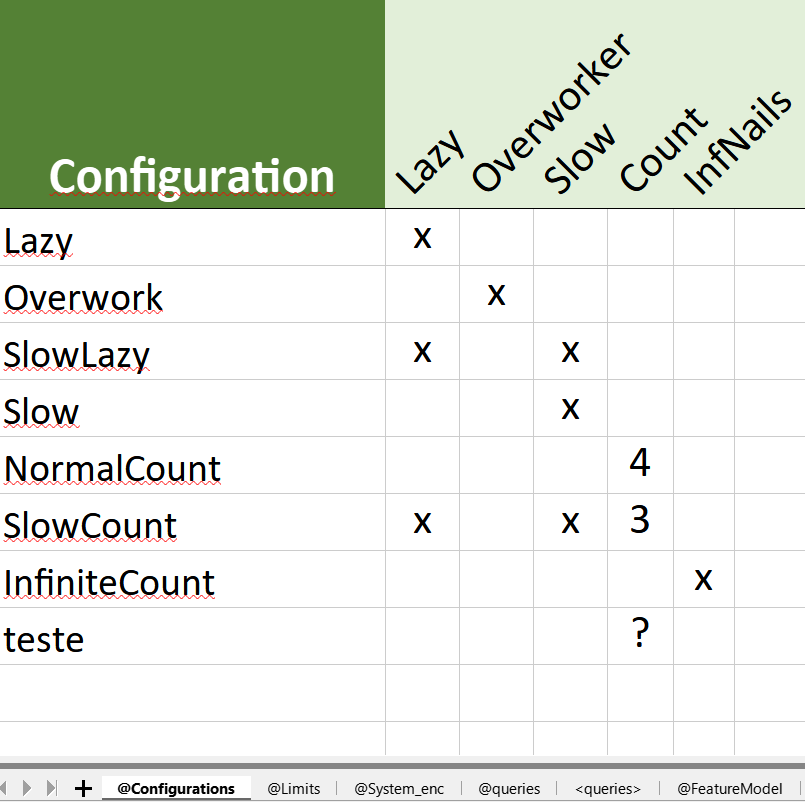
\includegraphics[width=0.8\linewidth]{images/newUp.png}};
            \begin{scope}[x={(image1.south east)},y={(image1.north west)}]
                \draw[black, thick] (0,0) rectangle (1,1); % coordenadas normalizadas
            \end{scope}
        \end{tikzpicture}
        \caption{Configurations Sheet Uppex}
        \label{fig:cof_WH}
    \end{minipage}
\end{figure}

As we can see in Figure \ref{fig:cof_WH}, the test configuration is a parametric configuration, with a ? in the product Count indicating its parametric nature. This can be interpreted as an uncertain or variable number selected for the Count product, unlike the previous configurations which have exact values.


\begin{figure}[H]
    \centering
    \begin{minipage}{0.48\textwidth}
        \centering
        \begin{tikzpicture}
            \node[anchor=south west,inner sep=0] (image1) at (0,0) {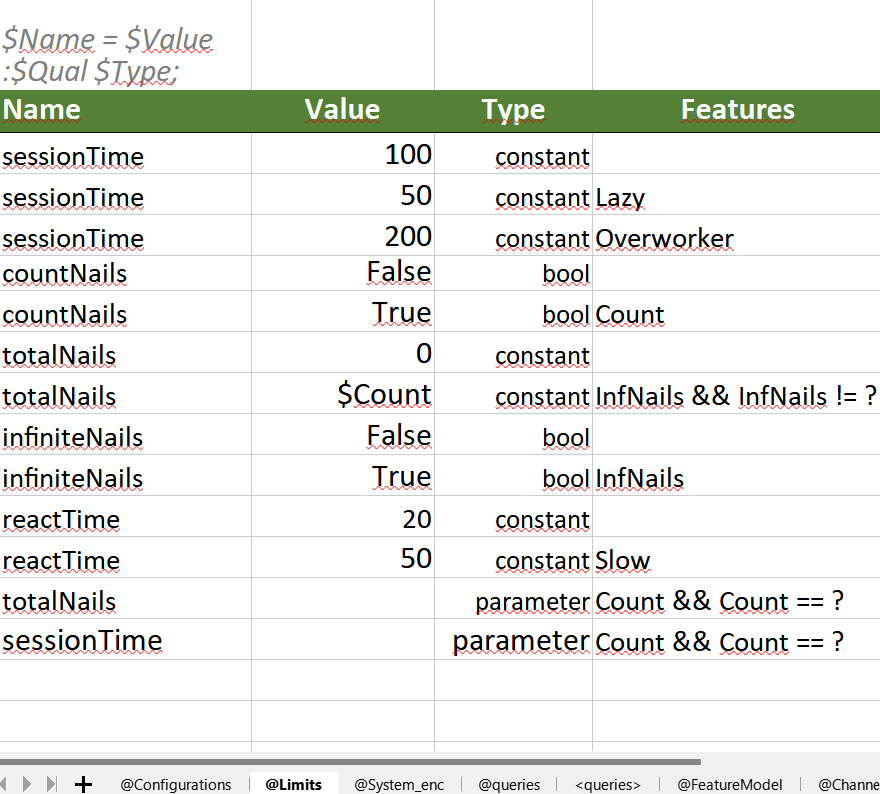
\includegraphics[width=\linewidth]{images/new_limits.png}};
            \begin{scope}[x={(image1.south east)},y={(image1.north west)}]
                \draw[black, thick] (0,0) rectangle (1,1); % coordenadas normalizadas
            \end{scope}
        \end{tikzpicture}
        \caption{Limits Sheet}
        \label{fig:PCSheet}
    \end{minipage}
    \hfill
    \begin{minipage}{0.48\textwidth}
        \centering
        \begin{tikzpicture}
            \node[anchor=south west,inner sep=0] (image2) at (0,0) {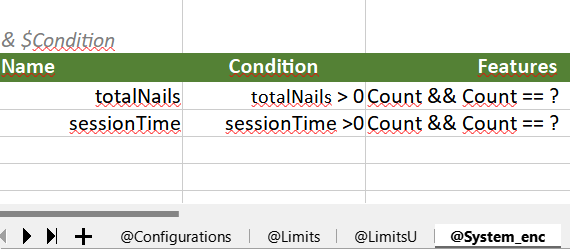
\includegraphics[width=\linewidth]{images/another_par.png}};
            \begin{scope}[x={(image2.south east)},y={(image2.north west)}]
                \draw[black, thick] (0,0) rectangle (1,1); % coordenadas normalizadas
            \end{scope}
        \end{tikzpicture}
        \caption{Parameters Constrain Sheet}
        \label{fig:LSheets}
    \end{minipage}
\end{figure}

In the test configuration, sessionTime and totalNails are introduced as parameters, as shown in Figure \ref{fig:PCSheet}, and the only condition imposed on these parameters is that they must be greater than 0, as seen in Figure \ref{fig:LSheets}. Additionally, the variable declaration pattern has changed compared to the previous version to accommodate the Imitator syntax.

Regarding the Queries Sheet Figure \ref{fig:cof_q}, in the non-parametric configurations that include the Lazy product, we check for the occurrence of deadlock. In the test configuration, in addition to this, we also verify the minimum value of the parameter totalNails required for the Work location in Worker to be reachable. Finally, the parameters constraint is checked to ensure that the NailDone location in Worker is reachable.


\begin{figure}[H]
    \centering
    \begin{minipage}{\textwidth}
        \centering
        \begin{tikzpicture}
            \node[anchor=south west,inner sep=0] (image1) at (0,0) {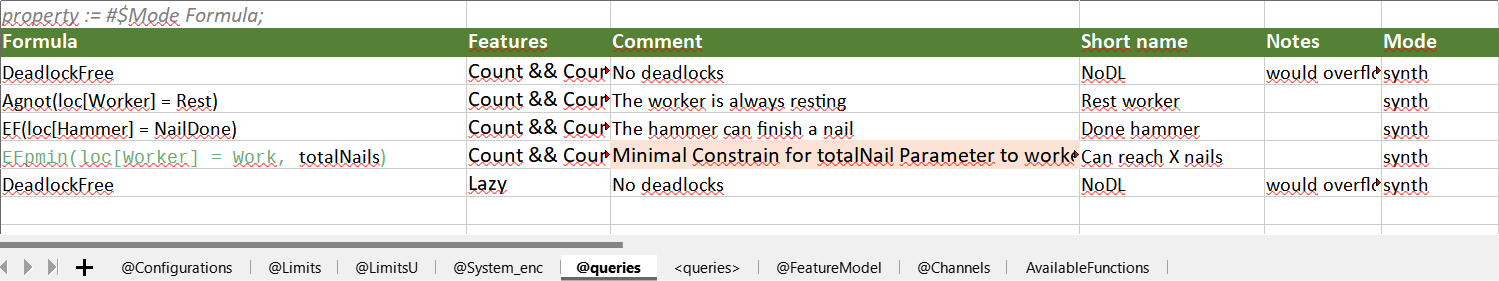
\includegraphics[width=\linewidth]{images/bla.png}};
            \begin{scope}[x={(image1.south east)},y={(image1.north west)}]
                \draw[black, thick] (0,0) rectangle (1,1); % coordenadas normalizadas
            \end{scope}
        \end{tikzpicture}
        \caption{Queries Sheet Uppex}
        \label{fig:cof_q}
    \end{minipage}
\end{figure}

With the updated Excel file, we move on to the parameterization of the .imi file that encapsulates our model. As previously explained, the annotation blocks are identified by the format \texttt{(*Name*)}. In this case, we will have two blocks: one for the variables, named \texttt{(*Limits*)}, and another for the parameter constraints, named \texttt{(*System\_enc*)}. For the non-parametric configurations, the Limits block will have the following structure:

\begin{verbatim}
    (*@Limits*)
    sessionTime = 100
    : constant;
    totalNails = 0
    : constant;
    countNails = True
    : bool;
    reactTime = 20
    : constant;
    infiniteNails = True
    : bool;
\end{verbatim}

Whereas in the test configuration, its content will differ due to the transformation of sessionTime and totalNails into parameters:

\begin{verbatim}
    (*@Limits*)
    countNails = True
    : bool;
    infiniteNails = False
    : bool;
    reactTime = 20
    : constant;
    sessionTime
    : parameter;
    totalNails
    : parameter;
\end{verbatim}


In the terminal, we use the command: \texttt{java -jar uppex.jar -runAll Imitator\_Model.imi}, thus compiling all configurations. The results can be seen in Appendix D. As previously explained, the groupby product and groupby requirement sections maintain the same format as the previous version; however, there is now a new type of result—specifically, the parametric interval, with an indication if an approximation has occurred. Finally, the new section includes the model image for each configuration, except for those not referenced in the queries sheet—that is, in the example, InfiniteCount, Main, NormalCount, Slow, and OverWork will remain empty.




















